\documentclass[12pt, a4paper, openany]{article}
\usepackage[utf8]{inputenc}
\usepackage[T1]{fontenc}

\usepackage{mfirstuc}

% LANGUAGE
\usepackage{enumitem}  % Enumerate improved

% MATH / Others
\usepackage{amsmath, amssymb}  % Math symbols
\usepackage{physics}  % \norm and \abs
\usepackage{esvect, cancel}  % Misc., vectors, strikethrough
\usepackage{mhchem}  % Chemistry
\usepackage{siunitx}  % Units SI
\usepackage{minted}  % Code fences ([cache=false])
\setminted[python]{
    fontsize=\footnotesize,
    tabsize=4,
    rulecolor=black,
    xleftmargin=18pt,
    linenos,
    breaklines
}
\usemintedstyle{pastie}

% GEOMETRY
\usepackage[
    paper=a4paper,
    top=2cm,
    left=2cm,
    headheight=15pt,
    headsep=12pt,
    textwidth=17cm,
    textheight=25.5cm,
]{geometry}
\usepackage{parskip}  % Reformat paragraphs, no indent first line
\usepackage{enumitem}  % Enumerate improved
\usepackage{scrextend}  % Indent text with addmargin environment
\usepackage{graphicx}  % Include graphics
\usepackage{wrapfig}
\graphicspath{{latex-img/}}
\usepackage{caption}  % Caption without figures
\usepackage{float}

\usepackage{paracol}

% HYPERLINKS
\PassOptionsToPackage{hyphens}{url}\usepackage{hyperref}
\hypersetup{
    colorlinks=true,
    linktoc=all,
    linkcolor=blue,
}
\usepackage{xurl}

\usepackage[bottom]{footmisc}

% HEADERS
\usepackage{fancyhdr}
    \pagestyle{fancy}
    \lhead{CS-358 MIT}
    \rhead{Helping Hand}
    \renewcommand{\footrulewidth}{0.4pt}
    \renewcommand{\headrulewidth}{0.4pt}
\usepackage{etoolbox}  % Define chapter page style
    \patchcmd{\chapter}{\thispagestyle{plain}}{\thispagestyle{fancy}}{}{}

% TITLE PAGE
\title{Helping Hand}
\author{Lucas Jung - IN BA6 324724\\Nour Guermazi - SC BA6 314474\\Pinar Oray - IN BA6 311543\\Jonas Sulzer - IN BA6 325554\\Yoan Giovannini IN BA6 303934}
\date{2024 - 03}


\newcommand{\footlink}[2]{\href{#2}{#1}\footnote{{\MakeUppercase #1}: \url{#2}}}
\newcommand*{\fullref}[1]{\hyperref[{#1}]{\autoref*{#1} \nameref*{#1}}}

\begin{document}
\maketitle
\thispagestyle{fancy}
\pagenumbering{arabic}

\begin{center}
    \textbf{Beyond Accessibility: Unleashing the Potential of Home Automation to Foster Independence and Inclusivity for Individuals with Unique Needs}
\end{center}

\par\noindent\rule{\textwidth}{0.4pt}
\vspace{-20pt}
\tableofcontents
\par\noindent\rule{\textwidth}{0.4pt}

\vspace{10pt}

\begin{minipage}[t]{0.65\textwidth}
    In the depicted image, you'll find Sean and Lucas.
    Sean, a colleague of Lucas' mother, is unfortunately grappling with \href{https://en.wikipedia.org/wiki/ALS}{amyotrophic lateral sclerosis}\footnotemark (ALS), a terminal neurodegenerative disease that progressively diminishes his mobility.
    Presently, he has to spend his days in an electric wheelchair, with only partial movement in his wrists.
    As a result, he relies on others for even the most basic tasks, such as opening a door or operating the lights in his home.
    Despite these challenges, Sean can still manage his smartphone while in his chair, thanks to a specialized joystick and a button.
    The objective of this project is to develop an adaptable solution that empowers people in a similar situation to regain some independence through the use of certain appliances in their home.
\end{minipage}\hfill
\begin{minipage}[t]{0.30\textwidth}
  \centering\raisebox{\dimexpr \topskip-\height}{
  \includegraphics[width=\textwidth]{human.jpg}}
\end{minipage}
\footnotetext{Amyotrophic Lateral Sclerosis: \url{https://en.wikipedia.org/wiki/ALS}}

\vspace{-10pt}

\section{High-level description}

The project aims to create a box in which the user can install any one of the various remote controls they have in their home.
The box will be equipped with a \footlink{plotter}{https://en.wikipedia.org/wiki/Plotter} like mechanism and a Wi-Fi capable microcontroller, allowing for remote operation of the enclosed remote control by having a solenoid activator attached to the plotter press on the buttons.
The box must be designed in such a way that the buttons are still usable without causing disruption to a user who prefers direct manual control of the remote.
The design of the case should also be easily adaptable to different type of remote controls.

Even though in the scope of the project we'll only be able to build one box, the idea is that a user can install multiple of these boxes for as many remotes as they want to use.
Each box is connected to the Wi-Fi network of the home it is installed in, and the user can command it by using an application on their smartphone.
Naturally, the application will be meticulously designed to maximize \footlink{accessibility}{https://en.wikipedia.org/wiki/Accessibility} for users with limited input capabilities.
Collaborative feedback and discussions with Sean will play a pivotal role in enhancing the system's accessibility, as he provides valuable insights from the perspective of a user with disabilities.

This project idea will be applied to some of the remote controlled appliances in Sean's home, notably in the two following use cases:
\begin{enumerate}
    \item In his residence, Sean has installed a motorized door (as seen behind us on the picture) that can be operated with a button press using a dedicated remote control, on which we could install the system.
        This holds significant importance for the project, as it would enable Sean to independently access his terrace and garden without relying on someone else to open the door for him.
    \item Additionally, he possesses remote-controlled blinds that he wishes to manage through his smartphone.
        This functionality would empower him to effortlessly close the blinds while working on his computer when the sun begins to shine through his window, or before going to bed.
\end{enumerate}

This project maintains its independence from specific use cases at Sean's place, aiming to be easily adaptable to most remote controls.
Nevertheless, establishing a direct connection and receiving periodic feedback from an end user like Sean during development significantly contributes to ensuring the system's accuracy and user-friendliness directly from the targeted audience.

Furthermore, the potential extends beyond Sean's specific needs: this system could serve as a prototype or a \footlink{minimal viable product}{https://en.wikipedia.org/wiki/Minimum_viable_product} (MVP)/pilot experiment for a cost-effective and easy to install commercial solution for a future startup company.
Such a solution would offer increased autonomy to numerous individuals in their daily lives.
It would be particularly competitive compared to existing alternatives that are very costly and often necessitate replacing the entire system with a ``smart``/digital version even though the one currently in place still works properly.
In fact, even though this system is targeted at people with disabilities, it might also come in handy for everyone who wishes to have access to their regular appliances through a common, digitalized interface.

A fundamental aspect of this project is its commitment to adhering to \footlink{open standards}{https://en.wikipedia.org/wiki/Open_standard} and the \footlink{open source}{https://en.wikipedia.org/wiki/Open_source} philosophy.
This commitment ensures the system's ease of customization for anyone interested in enhancing, tweaking, or adding functionalities.
This stands in stark contrast to existing solutions in the market, which are often characterized by closed systems that are challenging or even impossible to integrate into a accessible and simple to use central app and lack customization options.

\subsection{User Stories}

\begin{itemize}
    \item As a user with limited mobility, I want to independently open and close my motorized door using my smartphone, so I can access my terrace and garden without assistance.
    \item As a user who values autonomy, I want the modular box to be connected to the Wi-Fi network in my home, allowing me to control appliances remotely through my smartphone from anywhere in the house.
    \item As a user with a chronic degenerative disease affecting my mobility, I want to control my remote-controlled blinds via a smartphone app, allowing me to manage sunlight in my room without relying on others.
    \item As a user with unique needs, I want the modular box to be adaptable to different types of remote controls in my home, ensuring flexibility in controlling various appliances.
    \item As a potential end user looking for cost-effective solutions, I am looking for a commercial solution that offers increased autonomy, making it a viable and affordable option for individuals with diverse needs.
    \item As a developer or tech enthusiast, I want the system to adhere to open standards and open source philosophy, enabling me to enhance, customize, or add functionalities by making \footlink{pull requests}{https://en.wikipedia.org/wiki/Distributed_version_control} to the project's repository.
    \item As a user assisting someone with unique needs, I want the setup of the box and the configuration of the app to be straightforward and require minimal technical expertise, ensuring that I can provide support without complications even if I am not very skilled with new technologies.
    \item As a user with limited physical dexterity, I want to operate my TV remote control from my smartphone using the modular box system, allowing me to enjoy television without struggling with a conventional remote control.
\end{itemize}

\subsection{Existing Projects}

After searching online for existing solutions, Lucas discovered that none fully align with the objectives outlined above.
Many of the identified projects focus on complete replacement of the remote control, utilizing new emitters controlled by a microcontroller.
These implementations typically involve either \footlink{infrared emitters (project)}{https://github.com/computerjazz/ir-mobile} that record signals from the targeted remote control or \footlink{radio frequency (project)}{https://github.com/loopj/open-rts} based emitters that analyze the \footlink{rolling codes}{https://en.wikipedia.org/wiki/Rolling_code} of the initial device.

While these approaches are great and offer reliable performance, they are not well-suited for the inclusive and versatile goals of this project.
They often require installation on specific hardware and involve intricate setup and code manipulation to function.
This project aims to take a more broad and user-friendly approach by designing an adaptive solution that seamlessly integrates with various remote controls out of the box, whatever transmission mechanism they might use.

\section{Technical Specifications}

\textbf{Hardware Components}

The core of the modular box will utilize the \footlink{ESP32}{https://www.espressif.com/sites/default/files/documentation/esp32_datasheet_en.pdf} microcontroller for its compact size, low power consumption, and Wi-Fi capabilities.
This will enable seamless communication with the home network and the user's smartphone application.
Each box will be equipped with one ESP32 that will host and expose a \footlink{Web API}{https://en.wikipedia.org/wiki/Web_API} to interact with the plotter stepper motors and solenoid actuator from the smartphone application via the home Wi-Fi network.

The remote control will be housed in a laser-cut adjustable wood case/holding to accommodate various sizes and shapes.
The design should prioritize accessibility, ensuring that buttons remain accessible for direct manual control when needed.

Equipped with a plotter-like system, the box will simulate human interaction with the enclosed remote control.
This plotter system enables precise and controlled button presses, ensuring reliable functionality by moving to the exact position of the button and then actuating the button through a purely vertical movement done by the solenoid.

In a basic configuration process, after installing the remote in the box, the user selects button position by manually positioning the plotter using arrow buttons in the app.
The coordinate of that position is then saved and associated with a button and label in the app.

Additionally, to facilitate the setup process, an attachable module with a camera allows to assist the configuration of the device through computer vision.
If a user has multiple boxes in their home, they can use that single camera module to configure all of the boxes since it's only used during the setup process.
The computer vision, running on an external computer, also communicates over the network with the ESP32 board as well as with the camera to get the video feed.
The software detects the buttons on the image of the remote and allows the user to select the buttons to make available through the app.
For each of the chosen buttons, it auto-detects the exact position to execute the button press operation thanks to the visual feedback provided by the camera.
In case the user prefers not to use the camera and computer vision or in case the computer vision fails due to low contrast or a special remote type/design the manual setup process serves as a fallback. 

\begin{minipage}[t]{0.45\textwidth}
    \centering\raisebox{\dimexpr \topskip-\height}{
    \includegraphics[width=\textwidth]{latex-img/schema_top.png}}
\end{minipage}\hfill
\begin{minipage}[t]{0.5\textwidth}
    Looking from the top, we can see the base plate with the different components on it.\\

    Legend:
    \begin{itemize}
        \item (A) motors
        \item (B) rail (metal rod)
        \item (C) lead screw
        \item (D) base plate
        \item (E) solenoid holder
        \item (F) clamp
        \item (G) solenoid
        \item (H) wingnut
        \item (I) rubber
        \item (J) ESP32-c6
    \end{itemize}
\end{minipage}


\begin{minipage}[t]{0.5\textwidth}
    \begin{itemize}
        \item (K) ESP32-CAM
        \item (L) camera module
        \item (M) motor controller
        \item (N) power supply
        \item (P) solenoid controller
    \end{itemize}
    \vspace{5mm}

    From the side we can see how the plotter can move on the two axis hovering above the remote.
\end{minipage}
\begin{minipage}[t]{0.45\textwidth}
    \centering\raisebox{\dimexpr \topskip-\height}{
    \includegraphics[width=\textwidth]{latex-img/schema_front.png}}
\end{minipage}\hfill


\begin{minipage}[t]{0.45\textwidth}
    \centering\raisebox{\dimexpr \topskip-\height}{
    \includegraphics[width=\textwidth]{latex-img/schema_solenoid_holder.png}}
\end{minipage}\hfill
\begin{minipage}[t]{0.5\textwidth}
    \vspace{5mm}
    In the detail view of the solenoid holder we can see how the height of the solenoid can be adjusted to match the thickness of the remote.
\end{minipage}


\begin{minipage}[t]{0.5\textwidth}
    \vspace{5mm}
    The clamp allows to safely hold the remote in place.
\end{minipage}
\begin{minipage}[t]{0.45\textwidth}
    \centering\raisebox{\dimexpr \topskip-\height}{
    \includegraphics[width=\textwidth]{latex-img/schema_clamp.png}}
\end{minipage}\hfill


\begin{minipage}[t]{0.40\textwidth}
    \centering\raisebox{\dimexpr \topskip-\height}{
    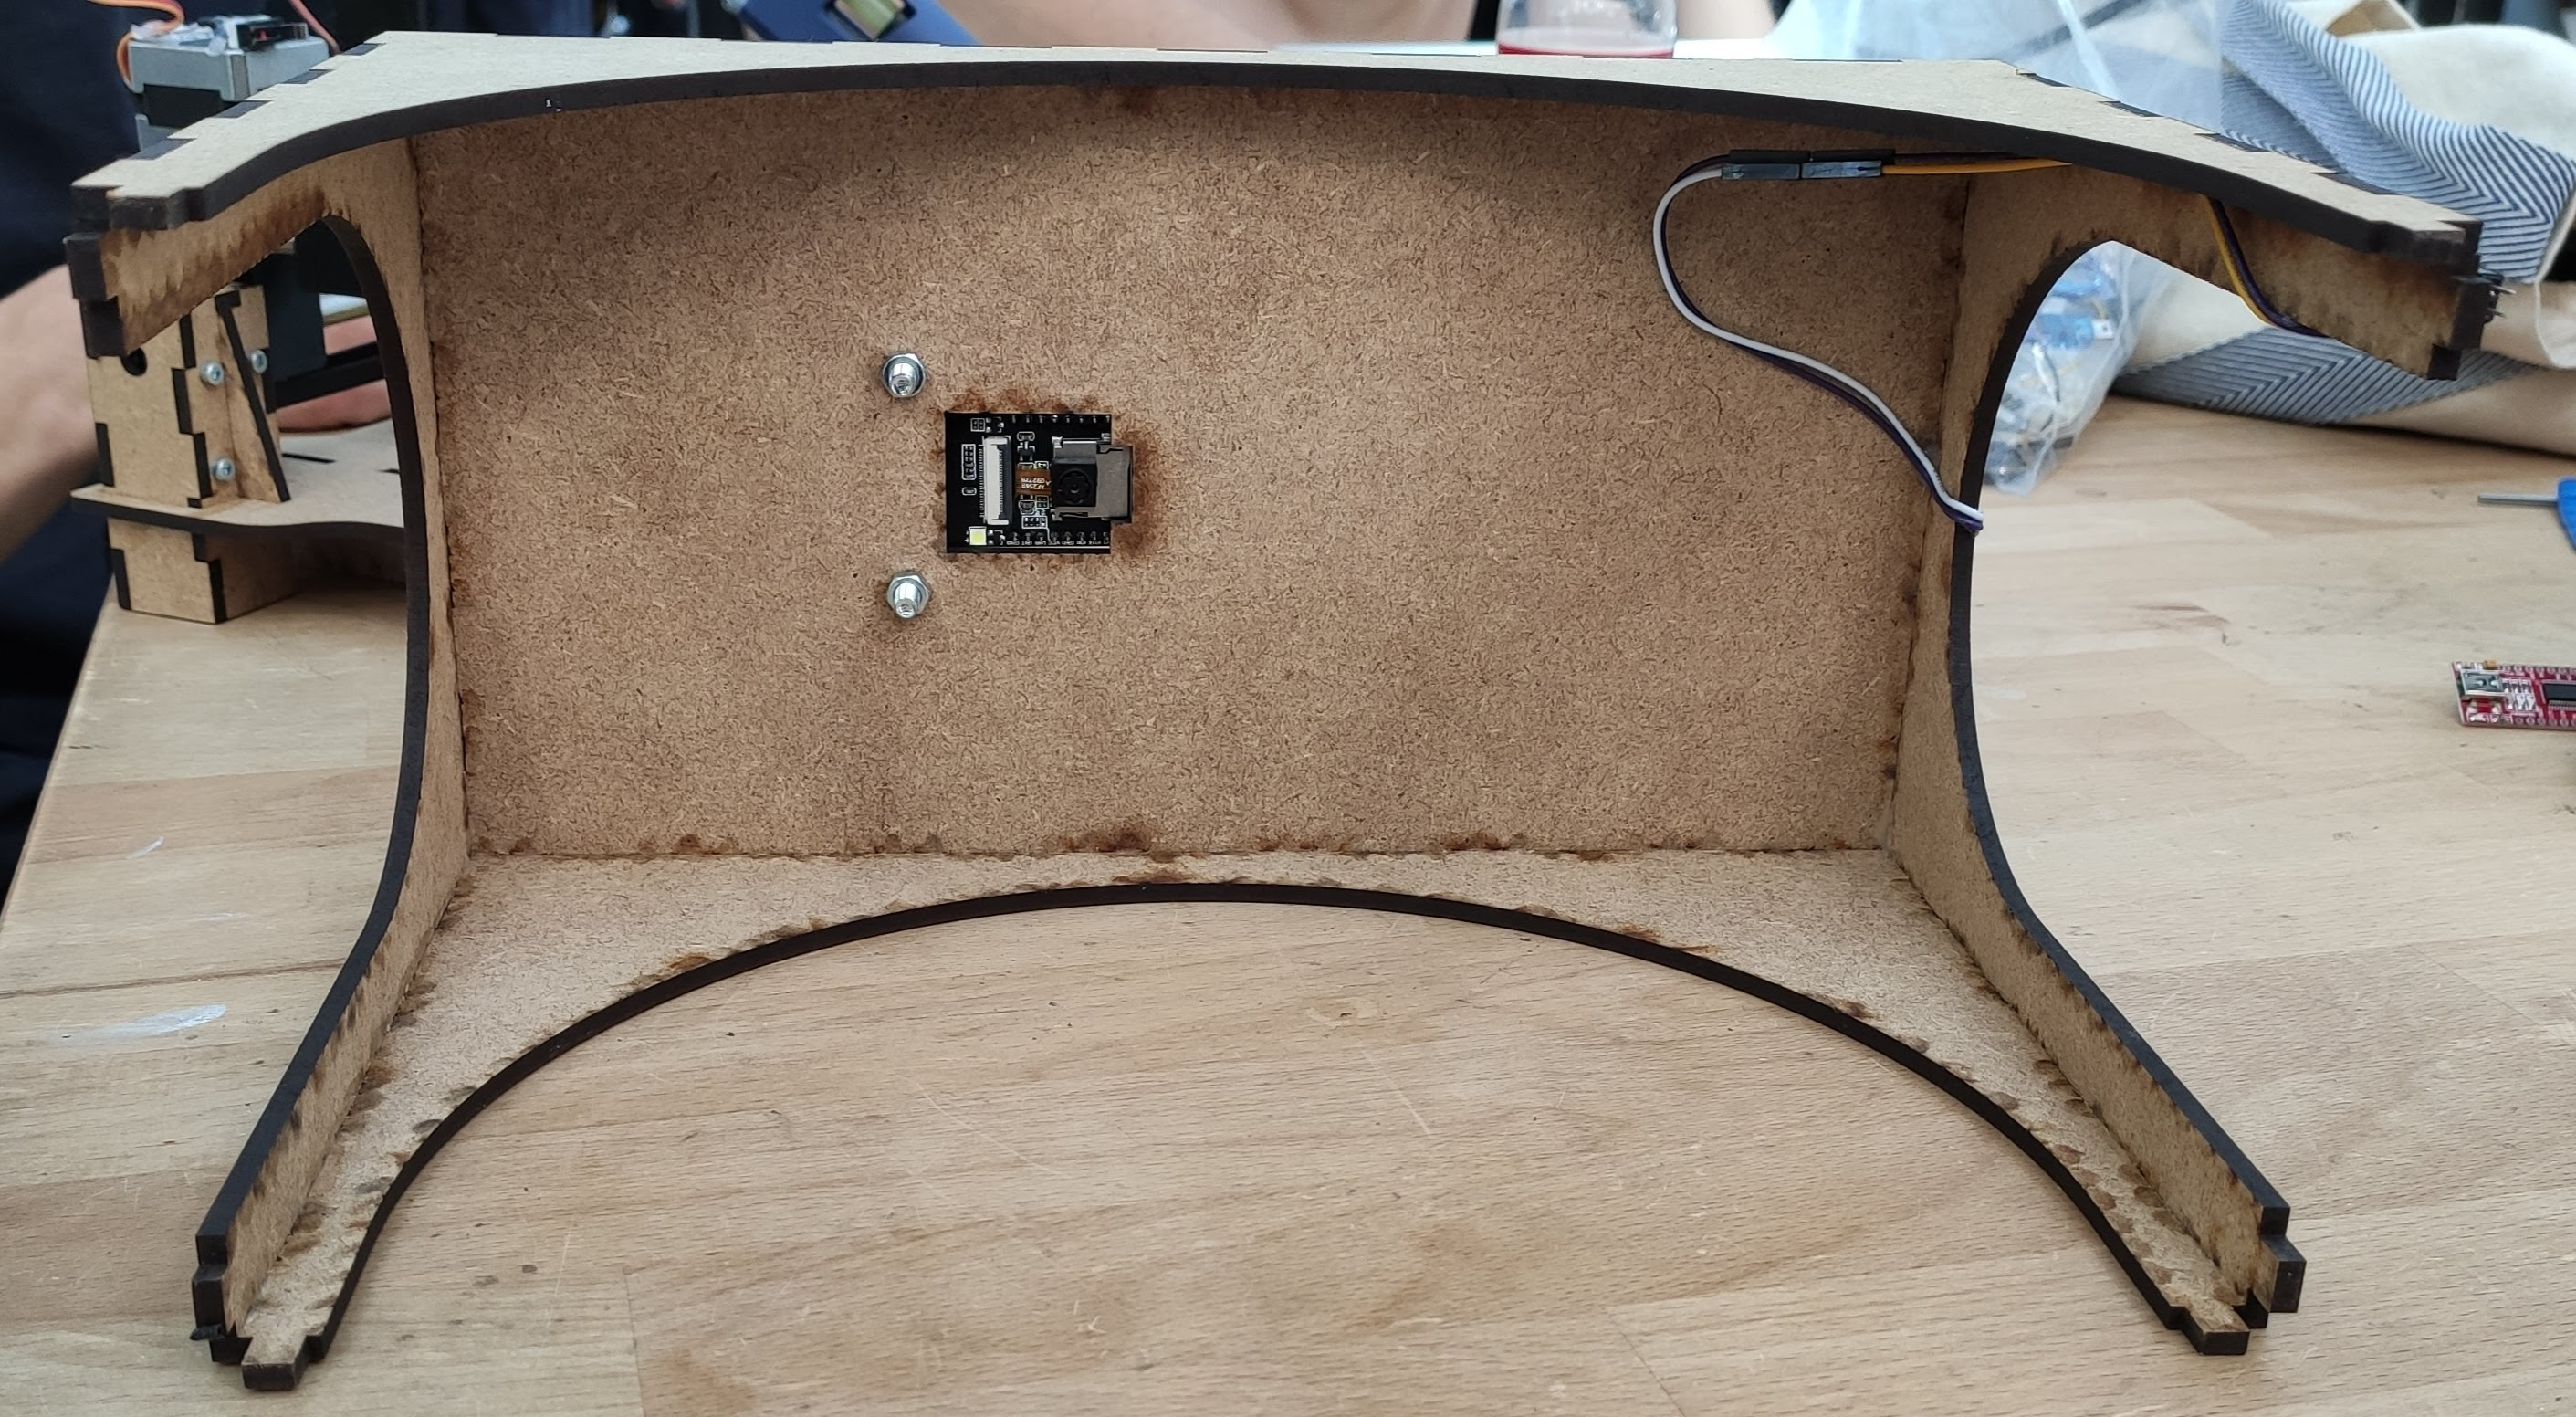
\includegraphics[width=\textwidth]{latex-img/camera_module.png}}
\end{minipage}\hfill
\begin{minipage}[t]{0.5\textwidth}
    \vspace{5mm}
    And finally the camera module.
\end{minipage}

\textbf{Software}

The software side of the project will be implemented using \footlink{Arduino}{https://www.arduino.cc/} programming to control the ESP32 microcontroller.
Arduino's user-friendly environment allows for efficient development and rapid iteration.

The dedicated smartphone application will be developed using the \footlink{Flutter framework}{https://flutter.dev/}.
The application will prioritize accessibility, offering a user-friendly interface tailored to individuals with limited input capabilities.
It should allow easy control of multiple boxes installed in the house.

The computer vision part is running on a computer assisting the setup. 
The application on the computer tries to recognize buttons on the remote and allows to easily choose the ones that should be accessible in the smartphone app.
When a button is selected, the computer vision calibrates the position for the button press and allows to test whether a button press actually works.
Finally, the configuration can be transferred to the smartphone by temporarily storing it on the ESP32.

We also need to design and implement an automatic network discovery protocol in order to automatically detect available remotes.
As we want to support many remote encasings in a single home network, the protocol has to assure correct communication between all the ESP32 boards and the smartphone application.

If time permits, we could enhance the application by incorporating a built-in voice controlled feature.
This addition would empower users to effortlessly command various devices using their voice, providing a more seamless experience.

\newpage
\section{Bill of Materials}

% TODO (gruvw)

\newpage
\section{Risk Assessment}

In this section, we conduct a comprehensive risk assessment to identify potential challenges and vulnerabilities that could impede the success of our project.
By evaluating technological risks we aim to proactively address these issues through strategic planning and prototype development.
This assessment underscores our commitment to ensure the resilience and adaptability of our project, thereby minimizing the likelihood of failure and maximizing its overall effectiveness.

% reword the below p
%  remote adaptability: required pressure for each remote is different: some hard-pressed, some don't require as much pressure to acknowledge a button press. another problem is that the remote sizes
%                         vary a lot in length but especially in width, which makes designing and creating a clamp that fixes most of the remotes difficult.  
%  calibration: the calibration as a first step is to be done manually, which would include manually moving the pushing mechanism to the button via the phone application and setting it up as a button. This might be somewhat 
%                 time consuming and hard to configure for non-technical users. 
%                 The next step to the setup includes computer vision.
%                 This also comes with its own challenges, and is complex because of the camera quality of the ESP32-CAM, the nature of remotes and the setup restrictions: small and non-tv remotes are likely to have similar colored buttons to 
%                 the remote's main body, and this makes recognition of individual buttons difficult. Another issue is that the setup, i.e. placing the remote in the clamp is done by a person, and this causes reliability issues
%                 in the sense that not everyone can place and clamp the remote perfectly, and this will cause a sligtly different placement each time. This will cause in a different lightning and a different angle of view for
%                 the camera to pick up. This might affect the accuracy of the image recognition. The computer vision part requires an external computer to set up button positions, and this information is then
%                 sent to the phone application, Here, the communication between the computer, the phone app and the plotter is crucial and complicated. 

\begin{itemize}
    \item Power supplies to steppers:\\
        As mentioned in the manual, inadequate wiring practices and carelessness may lead to frying a computer or damaging the parts, especially the motor drivers and the stepper motors, potentially putting at risk the functionality of the project.
    \item Control of the solenoid:\\
        While the solenoid allows for a completely vertical and uni-directional movement, since we don't have experience with them, we're not sure how precisely we can control the acceleration and force of the resulting movement.
        An alternative could be to use a stepper motor instead for pressing the remote buttons.\\
        An additional risk could be that not all buttons require the same pressure. It could be difficult to adapt to this.
    \item Adaptability to different remotes:\\
        The project's adaptability to different remote controls is a challenge, as compatibility issues may arise with various types of remotes due to the vast spectrum of sizes. The amount of different size and shapes possible makes it complicated to design the clamp mechanism. 
    \item Magnet interferences:\\
        The presence of magnets in the project could disrupt the operation of sensitive electronic components such as the solenoid push-down mechanism, motors or the WiFi chip of the ESP32, leading to unpredictable behavior.
    \item WiFi network stability:\\
        The reliance on WiFi connectivity on those ESP32 microcontrollers introduces a risk related to network instability, which could affect communication between project components.
    \item Ease of configuration:\\
        The configuration and calibration of the plotter will have the possibility to be done in two ways: manually via the phone app or with computer vision via a computer. The manual setup may be time consuming for remotes with many buttons. 
        The camera and computer vision setup may be hard to configure for non-technical users. This option also has its own additional challenges. The recogni̇ti̇on of the remote and its buttons rely on the camera, the placement of the remote, the lightning of the room
        and overall restrictions due to remote design. These may affect the accuracy of the image recognition.
    \item Computer vision to button press precision:\\
        Detecting the correct position and therefore being able to guarantee a precise button press while using computer vision to calibrate and configure the device could be difficult for the same reasons listed in above point.
\end{itemize}


\end{document}
